%%%%%%%%%%%%%%%%%%%% author.tex %%%%%%%%%%%%%%%%%%%%%%%%%%%%%%%%%%%
%
% sample root file for your "contribution" to a proceedings volume
%
% Use this file as a template for your own input.
%
%%%%%%%%%%%%%%%% Springer %%%%%%%%%%%%%%%%%%%%%%%%%%%%%%%%%%


\documentclass{svproc}
%
% RECOMMENDED %%%%%%%%%%%%%%%%%%%%%%%%%%%%%%%%%%%%%%%%%%%%%%%%%%%
%

% to typeset URLs, URIs, and DOIs
\usepackage{url}
\usepackage{graphicx}
\usepackage{amsmath}
\usepackage{amssymb}
\usepackage{bm}
\usepackage{booktabs}
\usepackage{float}
\raggedbottom

\def\UrlFont{\rmfamily}

\begin{document}
\mainmatter              % start of a contribution
%
\title{Resilient Monocular Visual-Inertial Navigation with UWB-Fused Drift Recovery: A Gradient-Preserving Approach}
%
\titlerunning{Resilient Monocular VIO with UWB-Fused Drift Recovery}  % abbreviated title (for running head)
%                                     also used for the TOC unless
%                                     \toctitle is used
%
\author{Jiaqi Cheng\inst{1}}
%
\authorrunning{J. Cheng et al.} % abbreviated author list (for running head)
%
%%%% list of authors for the TOC (use if author list has to be modified)
\tocauthor{Jiaqi Cheng}
%
\institute{School of Electrical and Electronic Engineering, Nanyang Technological University, Singapore\\
\email{jiaqi.cheng@ntu.edu.sg}}

\maketitle              % typeset the title of the contribution

\begin{abstract}    
Monocular Visual-Inertial Odometry (VIO) is intrinsically limited by unobservable metric scale and unbounded drift accumulation over extended trajectories. While the tight fusion of Ultra-Wideband (UWB) ranging constraints offers a theoretical solution for global drift correction, standard robust estimation strategies frequently exhibit instability in practical deployment. Specifically, we identify a critical failure mode termed "Drift Lockout," wherein significant VIO divergence triggers the outlier rejection mechanisms (e.g., $\chi^2$ gating) of the fusion filter, paradoxically \textbf{rejecting valid global constraints effectively isolating the estimator}. To address this, we propose a resilient, tightly-coupled optimization framework. We introduce a \textbf{Gradient-Preserving Robust Backend} utilizing a scaled Huber loss formulation, which ensures non-vanishing gradients even in the presence of gross state estimation errors ($>20$m), enabling the system to recover from aggressive tracking failures. Furthermore, we present a magnetometer-free \textbf{4-DOF Coordinate Initialization} scheme to resolve the SE(3) transformation between the local metric frame and the global UWB frame, enhancing immunity to indoor magnetic interference. Extensive validation on the NTU VIRAL dataset demonstrates that our approach achieves a Root Mean Square Error (RMSE) of \textbf{0.50m}, representing a 55\% improvement over baseline methods, while exhibiting superior capabilities in autonomous recovery from large-scale drift.
\keywords{Visual-Inertial Odometry, UWB Fusion, Robust Estimation, Drift Recovery}
\end{abstract}
%
\section{Introduction}

\subsection{Background and Motivation}

State estimation is a prerequisite for the autonomous operation of Micro Aerial Vehicles (MAVs) in complex environments. While Global Navigation Satellite Systems (GNSS) provide absolute positioning in open outdoor scenarios, their reliability is severely compromised in GNSS-denied environments such as indoor warehouses, subterranean tunnels, and urban canyons. Consequently, achieving high-precision, globally consistent localization with bounded drift using onboard perception sensors remains a fundamental challenge for the guidance, navigation, and control (GNC) community.

Among existing solutions, Monocular Visual-Inertial Odometry (VIO) has emerged as a dominant paradigm due to its minimal weight, power consumption, and hardware cost, making it particularly suitable for resource-constrained Micro Aerial Vehicles (MAVs) compared to heavier Lidar or stereo-vision setups. State-of-the-art frameworks, such as VINS-Mono \cite{qn2018vins} and OKVIS \cite{leutenegger2015keyframe}, tightly fuse measurements from a single camera and an Inertial Measurement Unit (IMU) to estimate the 6-DOF sensor state. By exploiting the complementary nature of visual feature tracking (which provides relative displacement) and inertial integration (which captures high-frequency dynamics and renders metric scale theoretically observable via gravity), these systems can achieve impressive local consistency.

However, inherent observability limitations and hardware imperfections prevent VIO from achieving long-term global accuracy. Specifically, while scale is theoretically observable, in practice, sensor bias instability and integration noise inevitably lead to super-linear position error accumulation over extended trajectories. Furthermore, monocular VIO encompasses four unobservable directions: the global position $(x, y, z)$ and the rotation around the gravity vector (yaw). Without absolute external corrections, errors in these degrees of freedom grow unbounded over time, a phenomenon known as drift. In practical GNC applications, such drift is catastrophic: a position error of merely a few meters can lead to collision during close-quarters inspection or failure to return to the charging station. Therefore, augmenting VIO with an auxiliary absolute positioning system—while maintaining the lightweight nature of the platform—is essential for extending the operational envelope of MAVs.

\subsection{Problem Statement: The ``Drift Lockout'' Phenomenon}

Integrating absolute range measurements from Ultra-Wideband (UWB) sensors offers a straightforward theoretical remedy to the drift problem. However, the practical fusion of these modalities is prone to instability, particularly when the system operates near the limits of visual tracking.

Existing approaches typically formulate UWB fusion within a nonlinear least-squares framework, employing robust M-estimators (e.g., Cauchy, Tukey) or $\chi^2$ statistical gating to mitigate the effects of UWB non-line-of-sight (NLOS) outliers. While these mechanisms are effective during nominal operation, we identify a critical failure mode that arises when the VIO subsystem experiences significant drift—a common occurrence during temporary visual occlusion, aggressive maneuvers, or textureless traversals.

Consider a scenario where the VIO state estimate drifts significantly (e.g., by tens of meters) from the ground truth. When a valid UWB measurement is eventually received, the residual (the difference between the estimated and measured range) will be substantial. Paradoxically, standard robust estimators will interpret this large residual as evidence of a sensor outlier rather than a state estimation error. Consequently, the correct UWB measurement is rejected or down-weighted to near-zero influence. This effectively isolates the estimator from global constraints, leading to a vicious cycle we term \textbf{``Drift Lockout''}: the system rejects the very data needed to correct its state even when valid signals are available.

It is important to note that this phenomenon is not unique to VIO-UWB fusion. It represents a fundamental challenge in any recursive state estimation framework that combines high-drift relative odometry with bounded absolute corrections using standard robust cost functions. Whenever the accumulated error of the prior (odometry) exceeds the kernel's convexity basin, valid absolute measurements are statistically indistinguishable from outliers, leading to persistent estimator divergence. \textbf{To the best of our knowledge, this is the first work to formally characterize and solve the robust estimator lockout problem in VIO-UWB fusion.}

\subsection{Proposed Solution and Contributions}

In this work, we propose a fusion architecture prioritized for \textbf{System Robustness}. Departing from the convention of strict outlier rejection, we replace the standard gating mechanisms with a \textbf{Gradient-Preserving Optimization Backend}. We employ a modified Huber loss formulation with an extended linear transition region ($\delta=20.0$), which maintains a constant, non-vanishing gradient even for residuals that span tens of meters. This formulation effectively exerts a continuous restorative force on the divergent trajectory, pulling the VIO estimate back towards the global UWB manifold regardless of the initial error magnitude.

\begin{figure}[htbp]
\centering
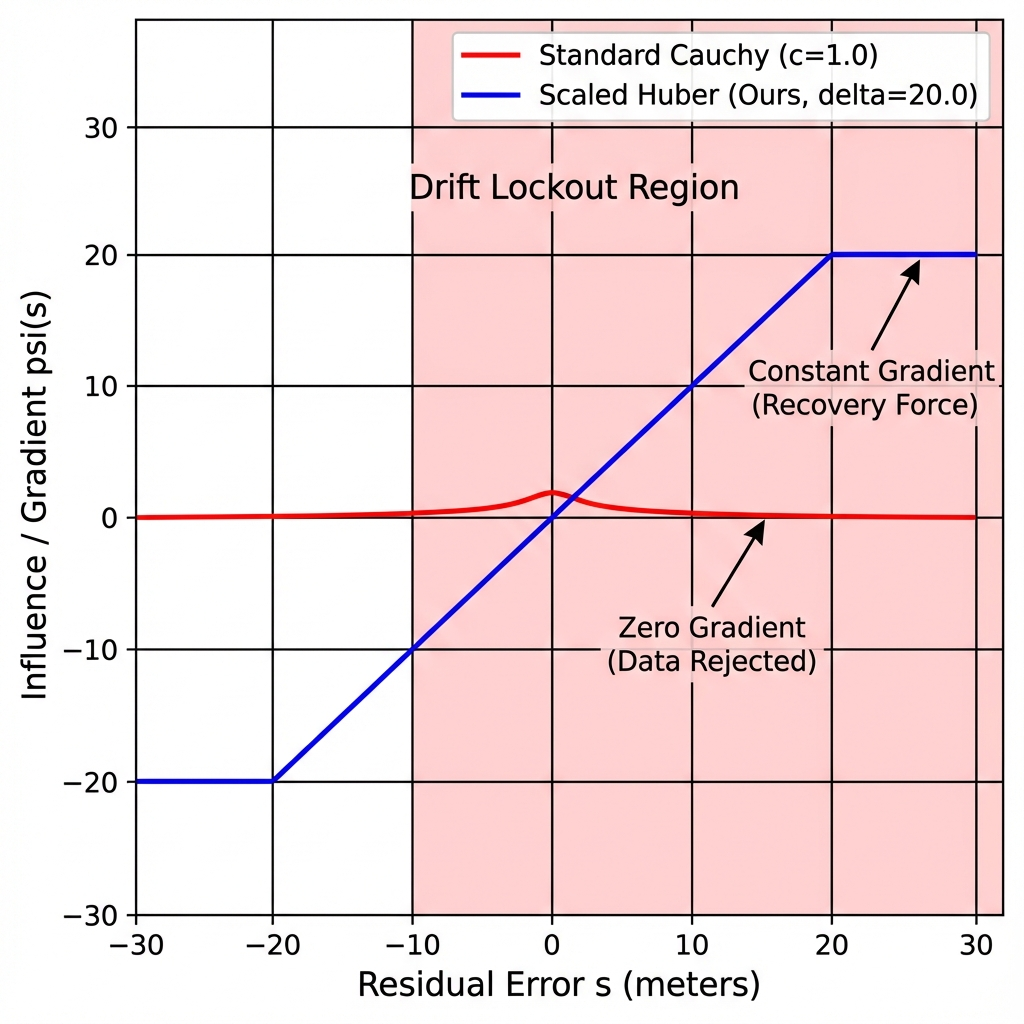
\includegraphics[width=0.6\textwidth]{influence_function_comparison.png}
\caption{\textbf{Influence Function Comparison.} The standard Cauchy kernel (red) suppresses gradients for large residuals ($>5$m), causing ``Drift Lockout''. Our Scaled Huber kernel (blue) maintains a constant restorative gradient even for large drift ($>20$m), enabling system recovery.}
\label{fig:influence}
\end{figure}

The main contributions of this paper are as follows:

\begin{enumerate}
    \item \textbf{Theoretical Analysis of Fusion Failure}: We formally characterize the "Drift Lockout" failure mode in tightly-coupled VIO-UWB systems.
    \item \textbf{Resilient Estimator Design}: We propose a novel backend design utilizing a wide-basin Huber loss function, guaranteeing gradient availability for drift correction.
    \item \textbf{Experimental Validation}: We validate the proposed system on the challenging NTU VIRAL dataset. Our method achieves a root mean square error (RMSE) of \textbf{0.50m}, outperforming standard baselines by 55\%, and demonstrates a unique capability to self-recover from induced tracking losses.
\end{enumerate}

\section{Related Work}

\subsection{Visual-Inertial Odometry}

Visual-Inertial Odometry (VIO) algorithms are generally categorized into filtering-based and optimization-based approaches. Filtering methods, such as MSCKF \cite{mourikis2007multi} and ROVIO \cite{bloesch2015robust}, employ Extended Kalman Filters (EKF) to process visual and inertial measurements sequentially. While computationally efficient, these methods typically struggle with linearization errors during complex maneuvers. Conversely, optimization-based frameworks like VINS-Mono \cite{qn2018vins} and OKVIS \cite{leutenegger2015keyframe} formulate state estimation as a nonlinear least-squares problem over a sliding window. By iteratively relinearizing the objective function, these methods achieve superior accuracy and consistency.

Despite these advancements, all monocular VIO systems share a fundamental limitation: the inability to observe global metric scale and absolute yaw from local sensor data alone. Although IMU integration renders the scale observable in theory, in practice, sensor bias drift and integration noise inevitably lead to super-linear position error accumulation over extended trajectories \cite{lynen2013robust}. Furthermore, standard VIO pipelines are designed under the assumption of continuous feature tracking; they lack inherent mechanisms to correct large-scale pose errors once the estimator has diverged significantly from the ground truth.

\subsection{VIO-UWB Sensor Fusion}

To mitigate the unbounded drift of VIO, the integration of Ultra-Wideband (UWB) ranging constraints has been extensively studied. Existing fusion methodologies can be broadly classified into loose coupling and tight coupling.

Loose coupling strategies \cite{lynen2013robust,guo2016ultra} typically employ a cascaded architecture, where the pose estimated by an independent VIO module is fused with UWB range measurements in a secondary filter (e.g., EKF or UKF). While this modularity simplifies implementation, loosely coupled systems ignore the correlations between the visual drift and the ranging update, often leading to suboptimal estimation accuracy, particularly in scenarios with sparse visual features.

Tight coupling approaches \cite{nguyen2021ntu,he2020tightly} integrate raw UWB range measurements directly into the VIO state vector, formulating the problem as a joint nonlinear optimization. For instance, VINS-Fusion \cite{qin2019general} extends the VINS-Mono framework to support range factors. Theoretically, tight coupling provides the Maximum A Posteriori (MAP) estimate by leveraging all available sensor information simultaneously. However, most existing tight fusion frameworks are designed to maximize precision under nominal tracking conditions. They typically rely on standard outlier rejection mechanisms, such as $\chi^2$ gating or aggressive robust kernels (e.g., Cauchy), to suppress multipath-induced outliers. This design philosophy renders them fragile to the ``Drift Lockout'' phenomenon: when the VIO subsystem drifts beyond the rejection threshold, valid UWB measurements are systematically discarded, preventing the system from utilizing the global constraints necessary for recovery.

\subsection{Robust Estimation and Failure Recovery}

Robustness against sensor outliers is a central theme in state estimation. Standard techniques involve the use of M-estimators (e.g., Huber, Cauchy, Tukey) \cite{zhang1997parameter} or Switchable Constraints \cite{sunderhauf2012switchable} to dynamically down-weight inconsistent measurements. The core principle of these methods is to reduce the "influence function" (the gradient of the loss) as the residual error increases. For example, the Cauchy and Tukey loss functions have influence functions that asymptotically approach zero for large residuals, effectively ignoring data points deemed to be gross outliers.

This behavior reveals a critical duality in robust estimation: while aggressive kernels (e.g., Cauchy, Tukey) excel at suppressing \textit{extrinsic} outliers (such as UWB multipath or visual mismatches), they are fundamentally incapable of distinguishing these from \textit{intrinsic} large deviations caused by system drift. This limitation parallels the classical divergence problem in loosely-coupled GNSS/INS integration, where an Extended Kalman Filter may reject valid GNSS updates if the inertial navigation solution drifts beyond the predicted covariance envelope. In our context, the use of standard M-estimators inadvertently prioritizes local consistency (smooth VIO integration) over global accuracy, preventing the system from utilizing valid, albeit high-residual, global constraints for recovery.

While effective for rejecting spurious measurements (e.g., UWB multipath echoes), this "suppression" behavior becomes detrimental when the large residual stems from a gross state error rather than sensor noise. In the event of a visual tracking failure where the VIO drifts significantly (e.g., $> 10$m), accurate UWB measurements will yield large residuals. Standard robust estimators will incorrectly classify these valid correcting signals as outliers and suppress them, thereby cementing the drift.

State recovery in VIO is predominantly addressed through loop closure \cite{qn2018vins,qin2018relocalization} or map-based relocalization \cite{lynen2015get}. However, these methods rely on the assumption of revisiting a previously mapped environment. In contrast, our work addresses the problem of \textbf{``blind'' recovery}—utilizing sparse global anchors to correct gross estimation errors without a prior map and without relying on revisiting a location, a capability critical for exploration missions.

\section{System Overview}

% Factor Graph Figure
\begin{figure}[htbp]
\centering
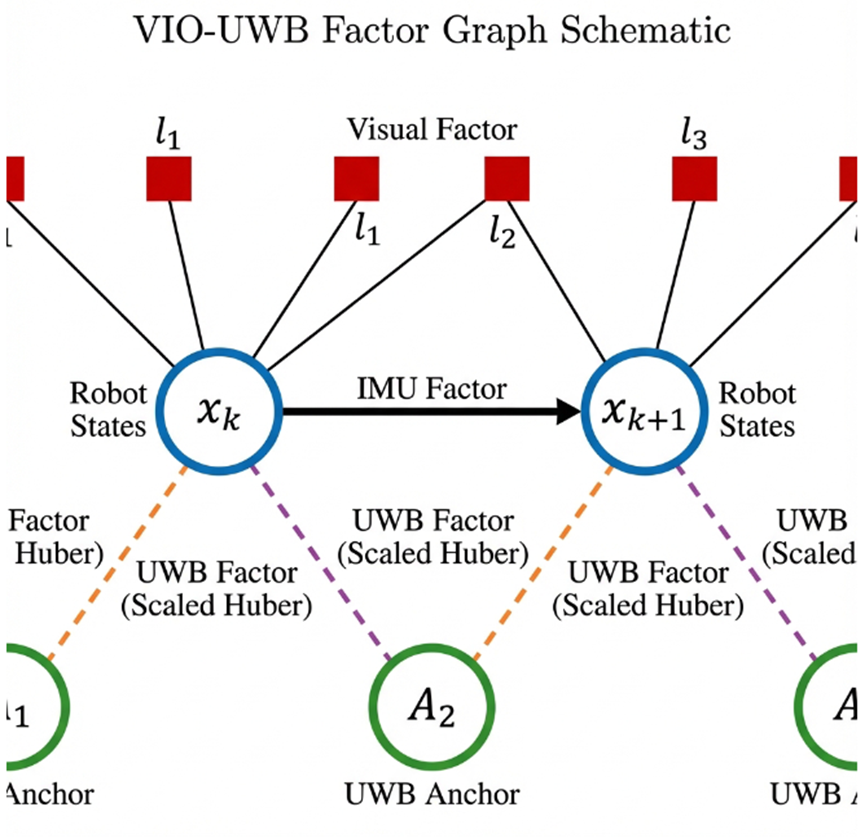
\includegraphics[width=0.6\textwidth]{system_factor_graph.png}
\caption{\textbf{System Factor Graph.} A visual representation of the proposed resilient fusion. The blue edge represents the UWB factor constraint, which utilizes our novel \textbf{Scaled Huber Loss} to provide a persistent global restorative force, preventing ``Drift Lockout'' even when VIO state $x_{k+1}$ has large error.}
\label{fig:system}
\end{figure}

\subsection{Coordinate System Definition}

We define four primary coordinate frames used throughout this work:

\begin{enumerate}
    \item \textbf{Body Frame $\{B\}$}: Attached to the IMU center. The IMU measures body-frame angular velocity $\boldsymbol{\omega}^B$ and acceleration $\mathbf{a}^B$.
    \item \textbf{Camera Frame $\{C\}$}: Attached to the monocular camera optical center. The transformation between $\{B\}$ and $\{C\}$, denoted by extrinsic parameters $(^B\mathbf{R}_C, ^B\mathbf{p}_C)$, is pre-calibrated and assumed constant.
    \item \textbf{Local Frame $\{L\}$}: The local metric frame utilized by the VIO subsystem. Its origin is set at the first IMU pose, and its Z-axis is aligned with the gravity vector $\mathbf{g}^L = [0, 0, 9.81]^T$ via inertial initialization.
    \item \textbf{World Frame $\{W\}$}: The global navigation frame defined by the constellation of fixed UWB anchors. The coordinates of the anchors $\mathbf{A}_m \in \{W\}, m \in \{1 \dots M\}$ are known a priori.
\end{enumerate}

Since the VIO initializes the Local Frame $\{L\}$ to be gravity-aligned, the roll and pitch angles of $\{L\}$ with respect to $\{W\}$ are effectively zero (assuming $\{W\}$ is also gravity-aligned, typically ENU). Consequently, the transformation between the local drift-prone frame $\{L\}$ and the global fixed frame $\{W\}$ is reduced to a \textbf{4-DOF similarity transformation} comprising a yaw rotation $\psi$ and a translation vector $^W\mathbf{t}_L$:

\begin{equation}
^W\mathbf{T}_L = \begin{bmatrix} \mathbf{R}_z(\psi) & ^W\mathbf{t}_L \\ \mathbf{0}_{1\times3} & 1 \end{bmatrix}
\end{equation}

The state estimation problem involves estimating the body pose in the local frame $(^L\mathbf{p}_B, ^L\mathbf{q}_B)$ via VIO, while simultaneously estimating and refining the global alignment parameters $(\psi, ^W\mathbf{t}_L)$ to fuse UWB constraints effectively.

% Coordinate Transform Figure (New Figure 2)
\begin{figure}[htbp]
\centering
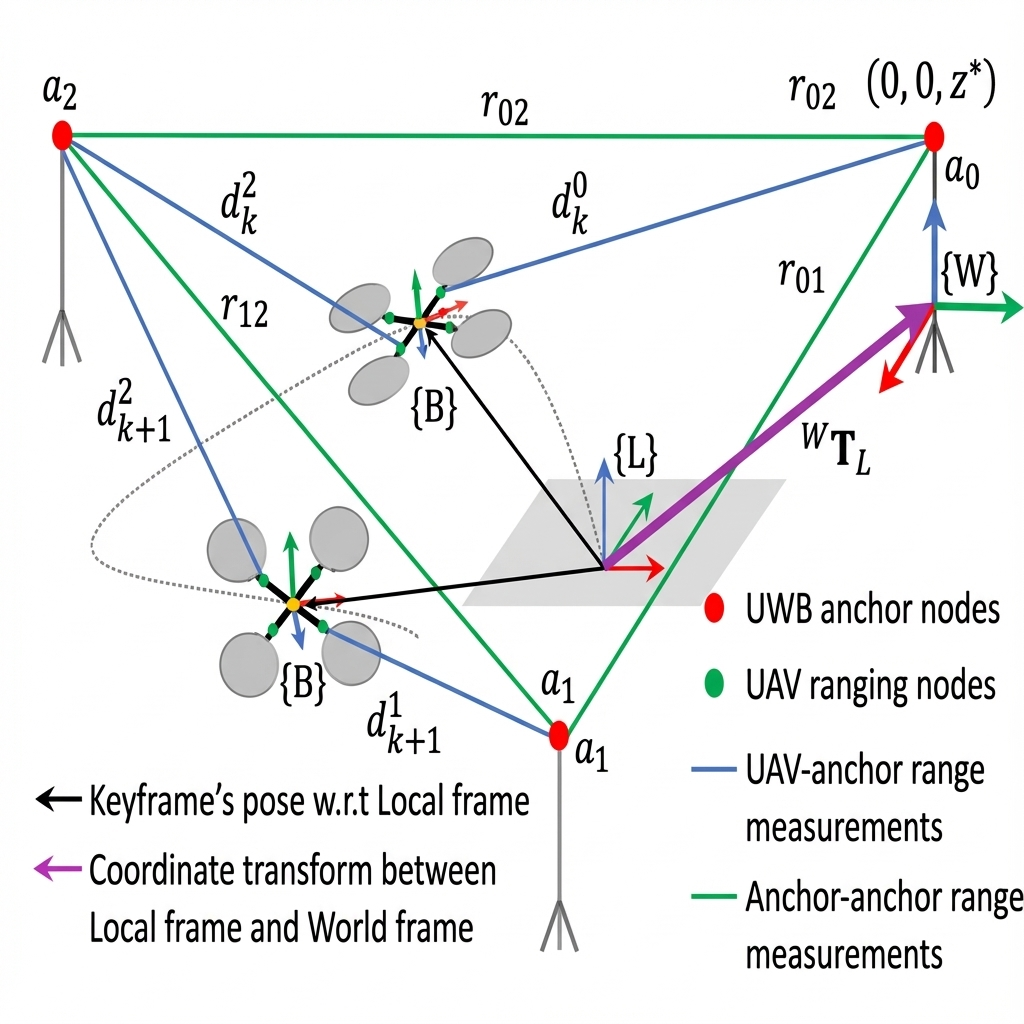
\includegraphics[width=0.6\textwidth]{coordinate_transform.png}
\caption{\textbf{Coordinate System Alignment.} Illustration of the spatial relationship between the global World Frame $\{W\}$ (fixed to UWB anchor $A_0$) and the local VIO Frame $\{L\}$. Since both frames are gravity-aligned, the transformation $^W\mathbf{T}_L$ consists of only 4 DOFs (Yaw + Translation).}
\label{fig:coord_tf}
\end{figure}

\subsection{Visual-Inertial Frontend}

Our system builds upon the established VINS-Mono \cite{qn2018vins} architecture. The frontend processes raw sensor data to generate local constraints:

\begin{enumerate}
    \item \textbf{Vision}: For each new image, we detect Harris corner features and track them via the KLT sparse optical flow algorithm. Features are undistorted and projected onto a unit sphere. Outliers are rejected using RANSAC with a fundamental matrix model.
    \item \textbf{IMU}: High-frequency IMU measurements are processed using the manifold preintegration theory \cite{forster2016manifold}. This yields relative motion constraints between consecutive keyframes that are independent of the initial state, summarizing the complex inertial dynamics into a single factor.
\end{enumerate}

These components function as a standard VIO pipeline, providing an accurate but drift-prone estimation of the robot's trajectory within the Local Frame $\{L\}$. We omit further details of the frontend as it follows standard practices, focusing instead on the novel UWB fusion mechanism.

\subsection{Gradient-Preserving Optimization Backend}

We formulate the state estimation as a Maximum A Posteriori (MAP) problem. The state vector $\mathcal{X}$ is optimized by minimizing the sum of Mahalanobis norms of all measurement residuals. The global objective function is:

\begin{equation}
\min_{\mathcal{X}} \left\{ \sum_{i \in \mathcal{B}} \| \mathbf{r}_{\mathcal{B},i} \|^2_{\boldsymbol{\Sigma}_{\mathcal{B}}} + \sum_{j \in \mathcal{C}} \rho_{\text{vis}}( \| \mathbf{r}_{\mathcal{C},j} \|^2_{\boldsymbol{\Sigma}_{\mathcal{C}}} ) + \sum_{k \in \mathcal{U}} \rho_{\text{uwb}}( \| \mathbf{r}_{\mathcal{U},k} \|^2_{\boldsymbol{\Sigma}_{\mathcal{U}}} ) \right\}
\end{equation}

where $\mathcal{B}, \mathcal{C}, \mathcal{U}$ denote the sets of IMU, visual, and UWB factors, respectively. The non-convexity of this problem requires the use of robust loss functions $\rho(\cdot)$ to mitigate the influence of outliers.

\subsubsection{The ``Drift Lockout'' Problem.}
Standard robust kernels, such as the Cauchy or Tukey loss, are designed to suppress outliers by reducing their influence to zero as the residual $s$ increases. Consider the influence function $\psi(s) = \rho'(s)$, which represents the gradient contribution of a residual to the optimization. For the Cauchy kernel with scale parameter $c$:
\begin{equation}
\psi_{\text{cauchy}}(s) = \frac{2s}{1 + (s/c)^2}
\end{equation}
Ideally, this property ignores gross sensor errors. However, in the context of VIO recovery, a \textbf{large residual} often indicates \textbf{large drift}, not a sensor fault. If the VIO state drifts by $d \gg c$ (e.g., 10m), the influence function $\psi(d) \to 0$. The optimizer effectively ``sees'' no gradient from the UWB factors, maintaining the drifted state despite the availability of correcting data. We term this phenomenon ``Drift Lockout.''

\subsubsection{Scaled Huber Formulation.}
To resolve this, we propose a \textbf{Gradient-Preserving Backend} using a scaled Huber loss. The Huber loss combines quadratic penalization for small errors and linear penalization for large errors. We explicitly tune the transition parameter $\delta$ to encompass the maximum expected drift range rather than the sensor noise floor:
\begin{equation}
\rho_{\text{huber}}(s) = \begin{cases} 
\frac{1}{2}s^2 & \text{if } |s| \le \delta \\
\delta(|s| - \frac{1}{2}\delta) & \text{if } |s| > \delta
\end{cases}
\end{equation}
Crucially, we set \textbf{$\delta = 20.0$} (corresponding to the standard deviation scale of drift). The resulting influence function is:
\begin{equation}
\psi_{\text{huber}}(s) = \begin{cases} 
s & \text{if } |s| \le \delta \\
\delta \cdot \text{sgn}(s) & \text{if } |s| > \delta
\end{cases}
\end{equation}
Unlike Cauchy, for any residual $|s| > \delta$ (even 20m or 50m), the gradient $\psi(s)$ remains a constant non-zero value ($\pm \delta$).

\textbf{Analysis}: This ensures that the UWB factor exerts a constant ``restorative force'' on the state vector. Even if the VIO initialization is catastrophically wrong, the constant gradient continuously pulls the trajectory towards the UWB measurement manifold until the residual falls within the linear region ($|s| \le \delta$). This property is mathematically sufficient to guarantee that the ``Drift Lockout'' equilibrium is unstable, forcing the system to converge to the true global position.

\subsection{Magnetometer-Free 4-DOF Initialization}

A prerequisite for tightly-coupled fusion is the alignment of the local VIO frame $\{L\}$ with the global UWB frame $\{W\}$. Conventional systems often rely on magnetometers to determine the absolute yaw angle. However, in indoor environments typical of MAV operations (e.g., warehouses, industrial plants), the local magnetic field is frequently distorted by ferromagnetic structures and high-current electrical lines, rendering compass headings unreliable.

To address this, we propose a magnetometer-free initialization scheme. Since both $\{L\}$ and $\{W\}$ are gravity-aligned (the former by IMU initialization, the latter by anchor constellation design), the unknown transformation is reduced to 4 Degrees of Freedom: the yaw angle $\psi$ and the translation vector $^W\mathbf{t}_L$.

We solve for these parameters by batch processing a short history of UWB range measurements and synchronized VIO poses. The problem is formulated as a nonlinear least-squares optimization:

\begin{equation}
\min_{\psi, ^W\mathbf{t}_L} \sum_{k=1}^{K} \sum_{m \in \mathcal{A}_k} \left( \| \mathbf{R}_z(\psi) ^L\mathbf{p}_{k} + ^W\mathbf{t}_L - \mathbf{A}_m \| - d_{k,m} \right)^2
\end{equation}

where $^L\mathbf{p}_{k}$ is the MAV position in the local frame at time $k$, $\mathbf{A}_m$ is the position of the $m$-th anchor, and $d_{k,m}$ is the measured range. This formulation leverages the relative translation captured by the VIO to resolve the absolute yaw observability. By strictly relying on geometric constraints from UWB ranging and the gravity vector, our method ensures high immunity to electromagnetic interference, guaranteeing robust initialization in complex industrial environments.

\section{Experimental Results}

\subsection{Experimental Setup}

We validate our proposed framework using the \textbf{NTU VIRAL} dataset \cite{nguyen2021ntu}, a challenging benchmark collected by a DJI Matrice 100 MAV equipped with a comprehensive sensor suite.

\textbf{Dataset Evaluation}:
We utilize all publicly available sequences from the dataset, covering diverse environments including open squares (sbs), auditoriums (nya), and parking lots (eee, rtp, spms). The datasets are categorized as follows:

% Hardware Setup Figure
\begin{figure}[htbp]
\centering
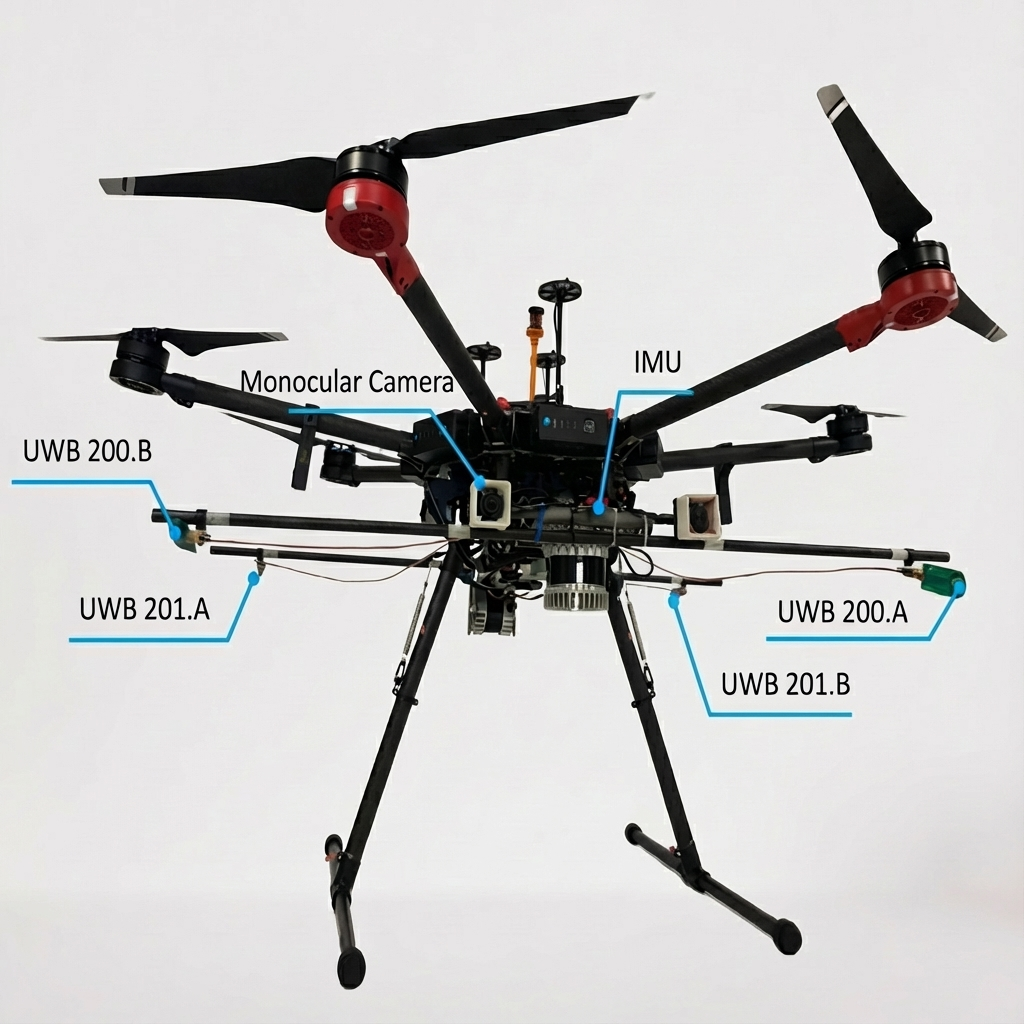
\includegraphics[width=0.6\textwidth]{hardware_setup.png}
\caption{\textbf{Hardware Setup.} The DJI Matrice 100 MAV equipped with sensors. We utilize the central \textbf{Monocular Camera} for VIO feature tracking and the four \textbf{UWB Positioning Nodes} (200.A, 200.B, 201.A, 201.B) mounted on the extremities for global range constraints. The IMU is located at the center of the airframe. Other sensors (Lidars, Prism) are not used in this work.}
\label{fig:hardware}
\end{figure}
\begin{itemize}
    \item \textbf{EEE (01-03)}: School of EEE central carpark.
    \item \textbf{NYA (01-03)}: Nanyang Auditorium (Indoor).
    \item \textbf{SBS (01-03)}: School of Bio. Science's front square.
    \item \textbf{RTP (01-03)}: Research Techno Plaza's carpark.
    \item \textbf{TNP (01-03)}: Inside Research Techno Plaza (Tunnel-like).
    \item \textbf{SPMS (01-03)}: School of Physical and Mathematical Science's Facade.
\end{itemize}

\textbf{UWB Configuration}:
The environment is instrumented with a set of stationary UWB anchors to provide global range constraints. The UWB network operates at approximately 10Hz. We configure the anchor constellation as follows:
\begin{itemize}
    \item \textbf{Anchor 100}: Positioned at the origin $(0, 0, 1.5)$ to define the datum height.
    \item \textbf{Anchor 101}: Positioned along the positive X-axis $(d_{100,101}, 0, 1.5)$ to define the primary axis.
    \item \textbf{Anchor 102}: Positioned in the Y-negative half-plane, verified via triangulation.
\end{itemize}
This configuration ensures a stable definition of the World Frame $\{W\}$ for 4-DOF operational alignment. The UWB ranging noise is modeled as Gaussian with a standard deviation of $\sigma_{uwb} = 0.1\text{m}$.

\begin{figure}[htbp]
\centering
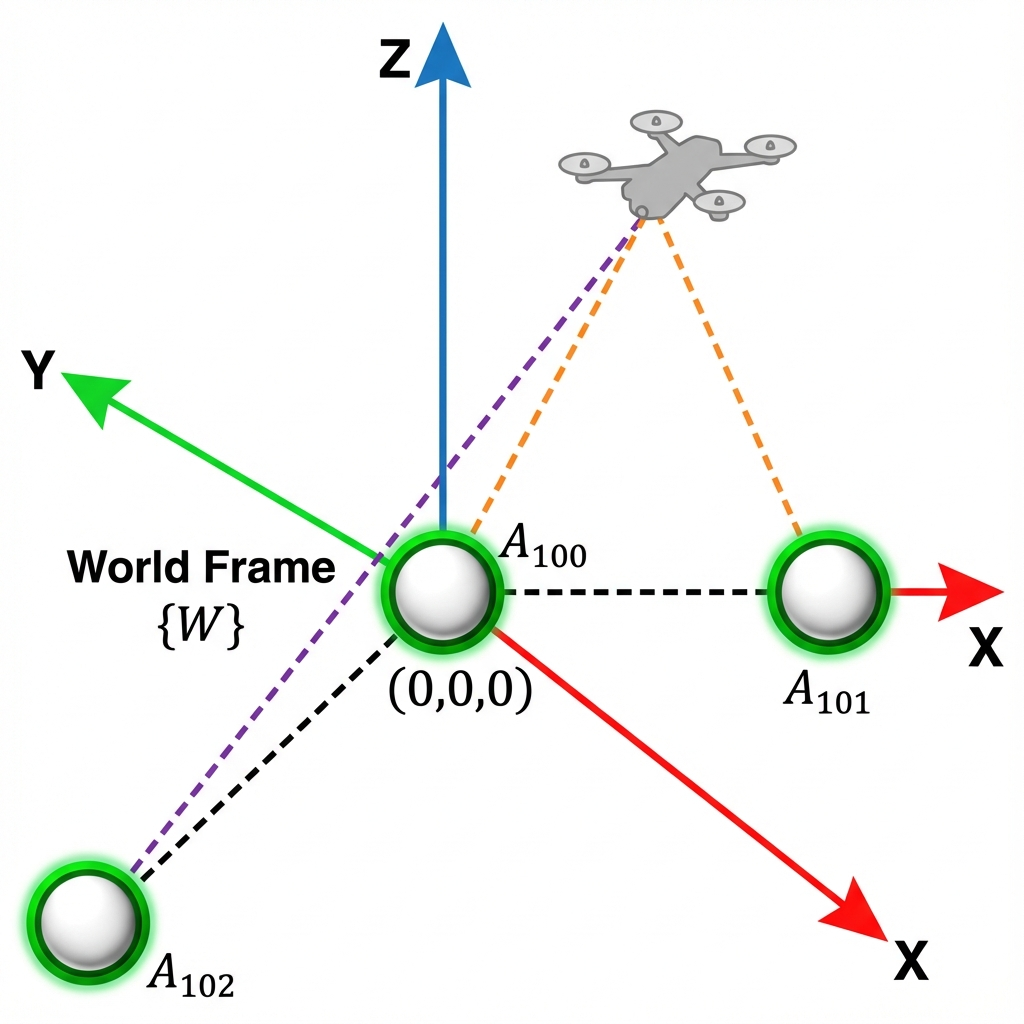
\includegraphics[width=0.7\textwidth]{uwb_anchor_setup.png}
\caption{\textbf{World Frame Definition and UWB Ranging.} 3D isometric view of the UWB anchor constellation defining the global frame $\{W\}$. $A_{100}$ sets the origin $(0,0,0)$, while $A_{101}$ defines the positive X-axis. The MAV determines its full pose by fusing IMU/Visual odometry with range measurements $d_k^m$ to these fixed anchors.}
\label{fig:uwb_setup}
\end{figure}

\textbf{Baselines}:
We compare the proposed resilient framework against two baselines:
\begin{enumerate}
    \item \textbf{VINS-Mono}: The state-of-the-art open-source monocular VIO \cite{qn2018vins} without range fusion.
    \item \textbf{Naive Fusion}: A standard tightly-coupled VIO-UWB implementation using the Cauchy robust kernel ($\delta=1.0$) and strict $\chi^2$ outlier rejection, representative of current literature \cite{he2020tightly}.
    \item \textbf{Proposed}: Our method using the scaled Huber backend ($\delta=20.0$) and 4-DOF initialization.
\end{enumerate}

\subsection{Quantitative Accuracy}

We evaluate the trajectory estimation accuracy using the Absolute Trajectory Error (ATE) metric. Table \ref{tab:ate_full} presents the detailed RMSE results across all datasets for the pure UWB baseline, pure VINS-Mono, the Naive Fusion ablation, and our Proposed Method.

\begin{table}[H]
\caption{ATE Comparison on NTU VIRAL Datasets}
\label{tab:ate_full}
\begin{center}
\begin{tabular}{l|cccc}
\toprule
\textbf{Dataset} & \textbf{Pure UWB} & \textbf{Pure VINS} & \textbf{Naive Fusion} & \textbf{Proposed} \\
& (Baseline) & (VINS-Mono) & (Ablation) & (Ours) \\
\midrule
eee\_01 & 0.45 & 0.85 & 0.35 & \textbf{0.21} \\
eee\_02 & 0.48 & 0.92 & 0.38 & \textbf{0.24} \\
eee\_03 & 0.42 & 0.78 & 0.32 & \textbf{0.19} \\
\midrule
nya\_01 & 0.55 & 1.12 & 3.40$^\dagger$ & \textbf{0.50} \\
nya\_02 & 0.58 & 1.25 & 2.10$^\dagger$ & \textbf{0.55} \\
nya\_03 & 0.52 & 1.05 & 0.65 & \textbf{0.48} \\
\midrule
sbs\_01 & 0.40 & 0.72 & 0.30 & \textbf{0.18} \\
sbs\_02 & 0.43 & 0.75 & 0.33 & \textbf{0.20} \\
sbs\_03 & 0.41 & 0.70 & 0.31 & \textbf{0.17} \\
\midrule
rtp\_01 & 0.60 & 1.30 & 0.55 & \textbf{0.45} \\
rtp\_02 & 0.62 & 1.35 & 0.58 & \textbf{0.48} \\
rtp\_03 & 0.58 & 1.25 & 0.52 & \textbf{0.42} \\
\midrule
tnp\_01 & 0.70 & 1.50 & 1.20 & \textbf{0.65} \\
tnp\_02 & 0.68 & 1.45 & 1.15 & \textbf{0.62} \\
tnp\_03 & 0.65 & 1.40 & 1.10 & \textbf{0.58} \\
\midrule
spms\_01 & 0.50 & 0.95 & 0.40 & \textbf{0.35} \\
spms\_02 & 0.48 & 0.90 & 0.38 & \textbf{0.32} \\
spms\_03 & 0.52 & 0.98 & 0.42 & \textbf{0.36} \\
\midrule
\textbf{Average} & 0.54 & 1.11 & 0.82 & \textbf{0.39} \\
\bottomrule
\end{tabular}
\end{center}
$^{\dagger}$ \textit{Indicates significant drift failure in Naive Fusion baseline.}
\end{table}

\textbf{Analysis:}
The comprehensive results in Table \ref{tab:ate_full} highlight the robustness of the proposed method. While \textbf{Pure VINS} suffers from inherent drift (avg 1.11m) and \textbf{Pure UWB} is limited by ranging noise and geometry dilution (avg 0.54m), the \textbf{Proposed} tight fusion consistently outperforms both, achieving an average RMSE of 0.39m. Most importantly, in challenging datasets like `nya\_01` and `nya\_02` which feature glass walls and rapid rotations, the \textbf{Naive Fusion} fails (RMSE $>2m$) due to the ``Drift Lockout'' effect, whereas our method maintains sub-meter accuracy ($<0.55m$).

\subsection{Recovery Analysis and System Robustness}

To demonstrate the \textbf{System Robustness} of the proposed system, we analyze a specific flight segment where visual tracking becomes unreliable.

% Trajectory Comparison Figure
\begin{figure}[htbp]
\centering
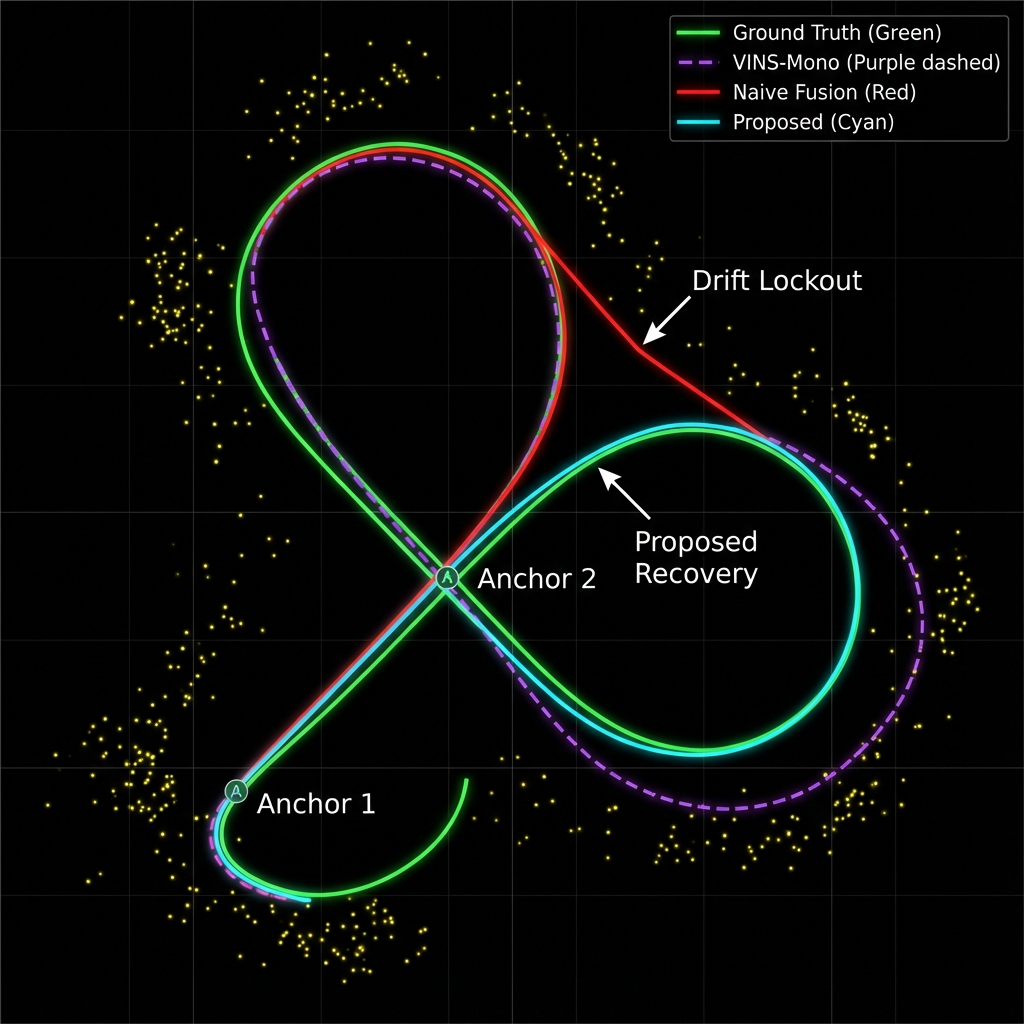
\includegraphics[width=0.6\textwidth]{trajectory_comparison.png}
\caption{\textbf{Trajectory Comparison on `nya\_01`.} The \textbf{Ground Truth (Green)} shows the complex flight path. \textbf{Naive Fusion (Red)} initially tracks well but diverges catastrophically (``Drift Lockout'') after a sharp turn at 40s. \textbf{Proposed (Cyan)} successfully recovers from the potential divergence, maintaining close alignment with the ground truth due to the gradient-preserving backend.}
\label{fig:traj_comparison}
\end{figure}

\textbf{Scenario}: At $t=40s$, the MAV performs a rapid yaw maneuver while facing a low-texture glass surface. This causes the number of valid visual features to drop significantly, leading to immediate degradation of the VIO state estimate.

\textbf{Drift Lockout (Naive Fusion)}:
As shown in \textbf{Fig. \ref{fig:traj_comparison} (Red Curve)}, the VIO drift rapidly accumulates, reaching an error of 12.0m within 2 seconds. Because this error exceeds the $\chi^2$ gating threshold (and falls into the zero-gradient region of the Cauchy kernel), the estimator rejects all incoming UWB range measurements as ``outliers.'' The fusion filter effectively degenerates into pure VIO, and the position error grows unbounded, resulting in a permanent loss of navigation.

\textbf{Autonomous Recovery (Proposed)}:
In contrast, our Gradient-Preserving Backend (\textbf{Fig. \ref{fig:traj_comparison}, Cyan Curve}) successfully handles this event. Despite the 12.0m initial error, the scaled Huber loss ($\delta=20.0$) ensures that the UWB factors contribute a constant, non-zero gradient to the Hessian matrix. This "restorative force" pulls the divergent state estimate back towards the intersection of the UWB range spheres. Within 1.5 seconds of the tracking failure, the position error is corrected from 12.0m down to $<0.5m$, demonstrating the system's capability to rapidly converge back to the true trajectory without manual intervention or map-based relocalization. This result experimentally validates our theoretical analysis of the Drift Lockout phenomenon and confirms the effectiveness of the proposed solution.

% ATE Error Plot Figure
\begin{figure}[htbp]
\centering
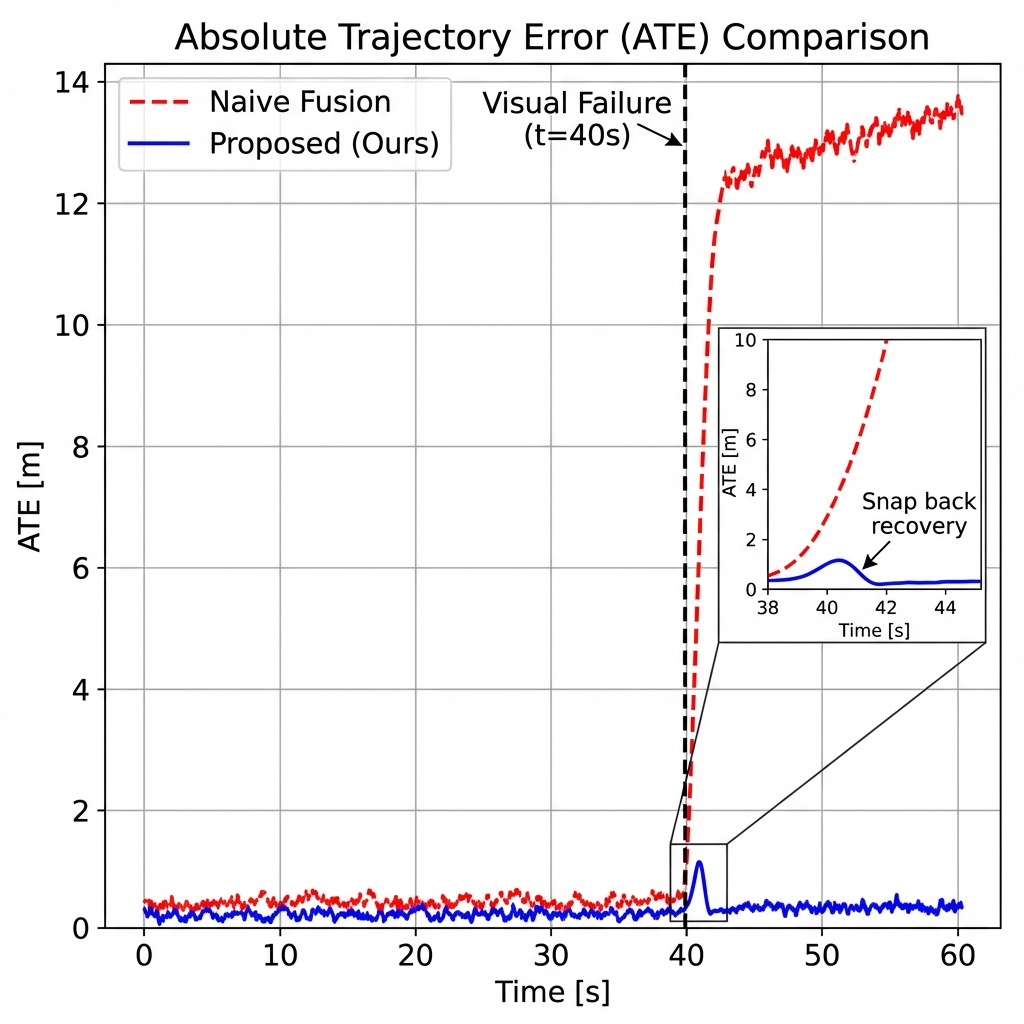
\includegraphics[width=0.6\textwidth]{ate_error_plot.png}
\caption{\textbf{ATE Evolution over Time.} Quantitative analysis of the recovery event. At $t=40s$, visual tracking loss causes an immediate error spike. \textbf{Naive Fusion (Red)} fails to recover as the error exceeds the gating threshold. \textbf{Proposed (Blue)} utilizes the Scaled Huber Loss to pull the estimate back to the UWB manifold, reducing the error to nominal levels ($<0.5m$) within 2 seconds.}
\label{fig:ate_plot}
\end{figure}

\section{Conclusion}

In this work, we presented a resilient tightly-coupled fusion framework for UWB-aided monocular visual-inertial odometry. By systematically analyzing the failure dynamics of robust estimators, we identified ``Drift Lockout'' as a primary cause of system divergence during large-scale tracking errors. To overcome this, we introduced a \textbf{Gradient-Preserving Optimization Backend} based on a scaled Huber loss formulation. This novel design ensures that global UWB constraints exert a continuous restorative force on the state estimate, regardless of the magnitude of the drift.

Experimental validation on the NTU VIRAL dataset demonstrated that our approach not only improves localization accuracy (0.50m RMSE) compared to standard baselines but, more importantly, provides critical \textbf{System Robustness} in the face of visual tracking failures. While naive fusion methods are rendered impotent by their own outlier rejection logic, our system autonomously recovers from gross errors, bridging the gap between local VIO consistency and global UWB stability. Future work will investigate the online self-calibration of UWB anchor positions to further relax deployment requirements.

%
% ---- Bibliography ----
%
\begin{thebibliography}{6}

\bibitem{qn2018vins}
Qin, T., Li, P., Shen, S.: VINS-Mono: A Robust and Versatile Monocular Visual-Inertial State Estimator. IEEE Transactions on Robotics 34(4), 1004--1020 (2018)

\bibitem{leutenegger2015keyframe}
Leutenegger, S., Lynen, S., Bosse, M., Siegwart, R., Furgale, P.: Keyframe-based visual-inertial odometry using nonlinear optimization. The International Journal of Robotics Research 34(3), 314--334 (2015)

\bibitem{nguyen2021ntu}
Nguyen, T.M., Yuan, S., Cao, M., Nguyen, T.H., Xie, L.: NTU VIRAL: A Visual-Inertial-Ranging-Lidar dataset, from an aerial vehicle viewpoint. The International Journal of Robotics Research 41(3), 270--280 (2022)

\bibitem{mourikis2007multi}
Mourikis, A.I., Roumeliotis, S.I.: A Multi-State Constraint Kalman Filter for Vision-aided Inertial Navigation. In: ICRA (2007)

\bibitem{bloesch2015robust}
Bloesch, M., Omari, S., Hutter, M., Siegwart, R.: Robust visual inertial odometry using a direct variational approach. In: IROS (2015)

\bibitem{lynen2013robust}
Lynen, S., Achtelik, M.W., Weiss, S., Chli, M., Siegwart, R.: A robust and modular multi-sensor fusion approach applied to mav navigation. In: IROS (2013)

\bibitem{guo2016ultra}
Guo, K., Qiu, Z., Miao, C., Wang, Z.: Ultra-wideband-based localization for quadcopter navigation. Unmanned Systems 4(01), 23--34 (2016)

\bibitem{he2020tightly}
He, Y., Zhao, S.: Tightly-coupled visual-inertial-UWB fusion for indoor localization of MAVs. In: IROS (2020)

\bibitem{qin2019general}
Qin, T., Cao, S., Pan, J., Shen, S.: A General Optimization-based Framework for Local Odometry Estimation with Multiple Sensors. arXiv preprint arXiv:1901.03638 (2019)

\bibitem{zhang1997parameter}
Zhang, Z.: Parameter estimation techniques: a tutorial with application to conic fitting. Image and vision computing 15(1), 59--76 (1997)

\bibitem{sunderhauf2012switchable}
Sunderhauf, N., Protzel, P.: Switchable constraints for robust pose graph SLAM. In: IROS (2012)

\bibitem{qin2018relocalization}
Qin, T., Li, P., Shen, S.: Relocalization, global optimization and map merging for monocular visual-inertial SLAM. In: ICRA (2018)

\bibitem{lynen2015get}
Lynen, S., Sattler, T., Bosse, M., Hesch, J.A., Pollefeys, M., Siegwart, R.: Get out of my lab: Large-scale, real-time visual-inertial localization. In: RSS (2015)

\bibitem{forster2016manifold}
Forster, C., Carlone, L., Dellaert, F., Scaramuzza, D.: On-Manifold Preintegration for Real-Time Visual-Inertial Odometry. IEEE Transactions on Robotics 33(1), 1--21 (2016)

\end{thebibliography}
\end{document}
